\documentclass[twoside]{article}

%
% ADD PACKAGES here:
%

\usepackage{amsmath,amsfonts,graphicx}
\usepackage[letterpaper, margin=1in]{geometry}

% Imports for writing pseudocode
\usepackage{algorithm}
\usepackage{listings}
\usepackage{xcolor}
\usepackage{graphicx,xspace}
\usepackage{enumerate}
\usepackage{enumitem}
\usepackage{booktabs}
\usepackage{mathtools}
\usepackage{tikz}
\usepackage{float}
\usepackage[colorinlistoftodos]{todonotes}
\definecolor{codegreen}{rgb}{0,0.6,0}
\definecolor{codegray}{rgb}{0.2,0.2,0.2}
\definecolor{background}{rgb}{0.95,0.95,0.92}
\lstdefinestyle{mystyle}{
    backgroundcolor=\color{background},
    commentstyle=\color{codegreen},
    keywordstyle=\color{blue},
    numberstyle=\tiny\color{codegray},
    basicstyle=\footnotesize,
    breakatwhitespace=false,
    breaklines=true,
    captionpos=b,
    keepspaces=true,
    numbers=left,
    numbersep=5pt,
    showspaces=false,
    showstringspaces=false,
    showtabs=false,
    tabsize=2
}
\lstset{style=mystyle}

%
% The following commands set up the lecnum (lecture number)
% counter and make various numbering schemes work relative
% to the lecture number.
%
\newcounter{lecnum}
\renewcommand{\thepage}{\thelecnum-\arabic{page}}
\renewcommand{\thesection}{\thelecnum.\arabic{section}}
\renewcommand{\theequation}{\thelecnum.\arabic{equation}}
\renewcommand{\thefigure}{\thelecnum.\arabic{figure}}
\renewcommand{\thetable}{\thelecnum.\arabic{table}}

%
% The following macro is used to generate the header.
%
\newcommand{\lecture}[4]{
   \pagestyle{myheadings}
   \thispagestyle{plain}
   \newpage
   \setcounter{lecnum}{#1}
   \setcounter{page}{1}
   \noindent
   \begin{center}
   \framebox{
      \vbox{\vspace{2mm}
    \hbox to 6.28in {{\bf CS 244	\hfill Spring 16-17}}
       \vspace{4mm}
       \hbox to 6.28in { {\Large \hfill Assignment #1: #2  \hfill} }
       \vspace{2mm}
       \hbox to 6.28in { {\it Professors: #3 \hfill Students: #4\/} }
      \vspace{2mm}}
   }
   \end{center}
   \markboth{Assignment #1: #2}{Assignment #1: #2}
}
%
% Convention for citations is authors' initials followed by the year.
% For example, to cite a paper by Leighton and Maggs you would type
% \cite{LM89}, and to cite a paper by Strassen you would type \cite{S69}.
% (To avoid bibliography problems, for now we redefine the \cite command.)
% Also commands that create a suitable format for the reference list.
\renewcommand{\cite}[1]{[#1]}
\def\beginrefs{\begin{list}%
        {[\arabic{equation}]}{\usecounter{equation}
         \setlength{\leftmargin}{2.0truecm}\setlength{\labelsep}{0.4truecm}%
         \setlength{\labelwidth}{1.6truecm}}}
\def\endrefs{\end{list}}
\def\bibentry#1{\item[\hbox{[#1]}]}

%Use this command for a figure; it puts a figure in wherever you want it.
%usage: \fig{NUMBER}{SPACE-IN-INCHES}{CAPTION}
\newcommand{\fig}[3]{
			\vspace{#2}
			\begin{center}
			Figure \thelecnum.#1:~#3
			\end{center}
	}
% Use these for theorems, lemmas, proofs, etc.
\newtheorem{theorem}{Theorem}[lecnum]
\newtheorem{lemma}[theorem]{Lemma}
\newtheorem{proposition}[theorem]{Proposition}
\newtheorem{question}[theorem]{Question}
\newtheorem{claim}[theorem]{Claim}
\newtheorem{corollary}[theorem]{Corollary}
\newtheorem{definition}[theorem]{Definition}
\newenvironment{proof}{{\bf Proof:}}{\hfill\rule{2mm}{2mm}}

% **** IF YOU WANT TO DEFINE ADDITIONAL MACROS FOR YOURSELF, PUT THEM HERE:
%Numbered environment
\newcounter{example}[section]
\newenvironment{example}[1][]{\refstepcounter{example}\par\medskip
   \noindent \textbf{Example~\thelecnum.\theexample. #1} \rmfamily}{\medskip}

\newcommand{\specialcell}[2][c]{%
 \begin{tabular}[#1]{@{}c@{}}#2\end{tabular}}

\newcommand\E{\mathbb{E}}

\begin{document}
%FILL IN THE RIGHT INFO.
%\lecture{**LECTURE-NUMBER**}{**TOPIC**}{**LECTURER**}{**SCRIBE**}
\lecture{2}{Congestion Control Contest}{K. Winstein \& S. Katti}{Jervis Muindi \& Luke Hsiao}

% **** YOUR NOTES GO HERE:

% Some general latex examples and examples making use of the
% macros follow.
%**** IN GENERAL, BE BRIEF. LONG SCRIBE NOTES, NO MATTER HOW WELL WRITTEN,
%**** ARE NEVER READ BY ANYBODY.

% \begin{figure}[H]
%   \caption{Example Cellphone SoC\label{fig:cell_soc}}
%   \centering
%     \includegraphics[page=5, trim={3cm 4cm 3cm 5.12cm}, clip, width=0.7\textwidth ]{lectures/07-flash-slides.pdf}
% \end{figure}

% \begin{algorithm}
% \caption{Discover Victim Cache}\label{victim}
% \begin{lstlisting}[language=C]
% char A[1024 * 64] = initialized;
%
% int baseline () {
%   sum = 0
%   // fill up cache with the first 32KB of A's data
%   for (int i = 0; i < 1024*32; i++) {
%   	sum += A[i];
%   }
%   sum += A[1024 * 32]; // cause cache conflict, load from main memory
%   return sum;
% }
% \end{lstlisting}
% \end{algorithm}


\section*{Exercise A}

\begin{question}
  Vary the fixed window size by editing controller.cc to see what happens.
  Make a 2D graph of throughput vs. 95-percentile signal delay (similar to what
  is seen on the contest analysis URLs) as you vary this value. What is the
  best single window size that you can find to maximize the overall "score"
  (log throughput/delay)? How repeatable are the measurements taken with the
  same window size over multiple runs?
\end{question}

We tried several different windows sizes in increments of 5 packets. The raw
numbers are shown in Table~\ref{tab:fixed_window}. Score is calculated as
$throughput / delay$, and the best score is shown in bold.

\begin{table}[h]
  \centering
  \caption{Throughput and Delay vs Fixed Window Size}
  \label{tab:fixed_window}
  \scriptsize
\begin{tabular}{rrrr}
  \toprule
  \textbf{\specialcell{Window\\Size}} & \textbf{\specialcell{Throughput\\(Mbits/s)}} & \textbf{\specialcell{95\% Signal\\Delay (ms)}} & \textbf{Score}\\
  \midrule
  5                           & 1.05          & 109          & 9.63           \\
  10                          & 1.93          & 155          & 12.45          \\
  \textbf{15}                 & \textbf{2.66} & \textbf{212} & \textbf{12.55} \\
  20                          & 3.26          & 277          & 11.77          \\
  25                          & 3.73          & 343          & 10.87          \\
  30                          & 4.07          & 401          & 10.15          \\
  35                          & 4.32          & 453          & 9.54           \\
  40                          & 4.51          & 504          & 8.95           \\
  45                          & 4.65          & 557          & 8.35           \\
  50                          & 4.76          & 607          & 7.84           \\
  55                          & 4.85          & 652          & 7.44           \\
  60                          & 4.91          & 711          & 6.91           \\
  65                          & 4.94          & 763          & 6.48           \\
  70                          & 4.96          & 808          & 6.13           \\
  75                          & 4.98          & 855          & 5.82           \\
  80                          & 4.99          & 896          & 5.57           \\
  85                          & 5.00          & 935          & 5.34           \\
  90                          & 5.00          & 972          & 5.14           \\
  \bottomrule
\end{tabular}
\end{table}

These values are plotted as a 2D graph of throughput vs 95-percentile signal
delay in Figure~\ref{fig:throughput_delay}.

\begin{figure}[h]
  \centering
  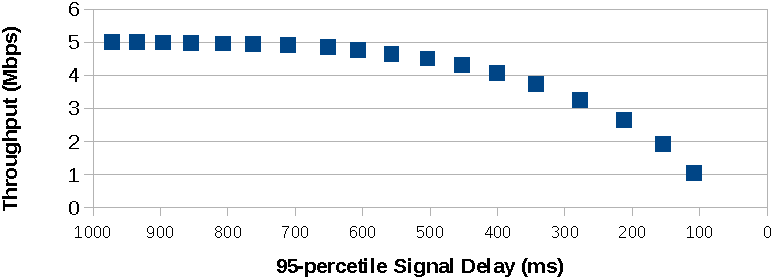
\includegraphics[height=3cm]{./img/exa_throughput_delay.pdf}
  \caption{Throughput vs 95-percentile Signal Delay for varying fixed window size.}
  \label{fig:throughput_delay}
\end{figure}

To answer the questions, we found that the best score was at a fixed window
size of about 15 packets. The measurements taken with the same window size
over multiple runs were very repeatable, in the mahimahi environment. The
throughput and delays only varied slightly (i.e. $\pm$ a few hundredths of Mbps
or a few ms).

\vfill
\pagebreak

\section*{Exercise B}
\begin{question}
  Implement a simple AIMD scheme, similar to TCP's congestion-avoidance phase.
  How well does this work? What constants did you choose?
\end{question}

For this exercise, we implemented a simple AIMD protocol, which increments the
\texttt{cwnd} by $alpha/cwnd$ on each ack, and decreases the window by
\texttt{beta} on a loss event (i.e. $cwnd = cwnd / beta$).
This mimics the AIMD behavior of TCP in congestion avoidance.
In our mahimahi environment, there is no loss, and there is unbounded queues.
Thus, to signal when a multiplicative decrease should occur, we use a fixed
timeout value as a signal. We set the timeout to 80ms, which is approximately
the 95-percentile signal delay on the top algorithms from the leaderboard.
We also set the initial congestion window size to 10.

We tried a few of different values for \texttt{alpha} and \textff{beta},
and recorded their performance in Table~\ref{tab:aimd}.

\begin{table}[h]
  \centering
  \caption{Throughput and Delay for for various AIMD constants}
  \label{tab:aimd}
  \scriptsize
  \begin{tabular}{rrrrr}
    \toprule
    \textbf{Alpha} & \textbf{Beta} & \textbf{\specialcell{Throughput\\(Mbits/s)}} & \textbf{\specialcell{95\% Signal\\Delay (ms)}} & \textbf{Score}\\
    \midrule
    1              & 2            & XXX                             & XXX & XXX \\
    \bottomrule
  \end{tabular}
\end{table}

We found that [stuff]

\vfill
\pagebreak

\section*{Exercise C}
\begin{question}
  Implement a simple delay-triggered scheme, where the window rises or falls
  based on whether the round-trip-time crosses some threshold value. Experiment
  with a few thresholds or tweaks and report on what worked the best.
\end{question}

\section*{Exercise D}
\begin{question}
  Try different approaches and work to maximize your score on the final
  evaluation. Be wary about "overtraining": after the contest is over, we
  will collect new network traces and then run everybody's entries over the
  newly-collected evaluation trace. In your report, please explain your
  approach, including the important decisions you had to make and how you made
  them. Include illustrative plots.
\end{question}
\section*{Exercise E}
\begin{question}
  Pick a cool name for your scheme!
\end{question}


% =============================================================================
\end{document}
